\chapter{Sistema de reconocimiento de gestos propuesto}\label{capit:cap3}
\vspace{-2.0325ex}%
\noindent
\rule{\textwidth}{0.5pt}
\vspace{-5.5ex}% 
\newcommand{\pushline}{\Indp}% Indent puede ir o no :p

En este cap\'itulo se describe el sistema de reconocimiento de gestos propuesto, este consta de cuatro etapas principales. La primera etapa es la adquisición de los datos, en la cual se capturan las imágenes de entrada del sistema; la segunda etapa es la detección aquí la mano es localizada y segmentada del fondo; en la etapa tres se extraen las características de la mano para ser procesadas en la etapa final donde el gesto realizado es reconocido. 

\section{Adquisición de los datos}\label{sec:AdquisicionDatos}

En esta etapa se capturan los datos que son la entrada del sistema. Los datos provienen de los sensores de profundidad de dos dispositivos Kinect, estos se encuentran ubicados uno frente al  usuario y otro al lado  izquierdo como se muestra en la figura \ref{fig:SetupSystem}.

\begin{figure}[!h]
\begin{center}
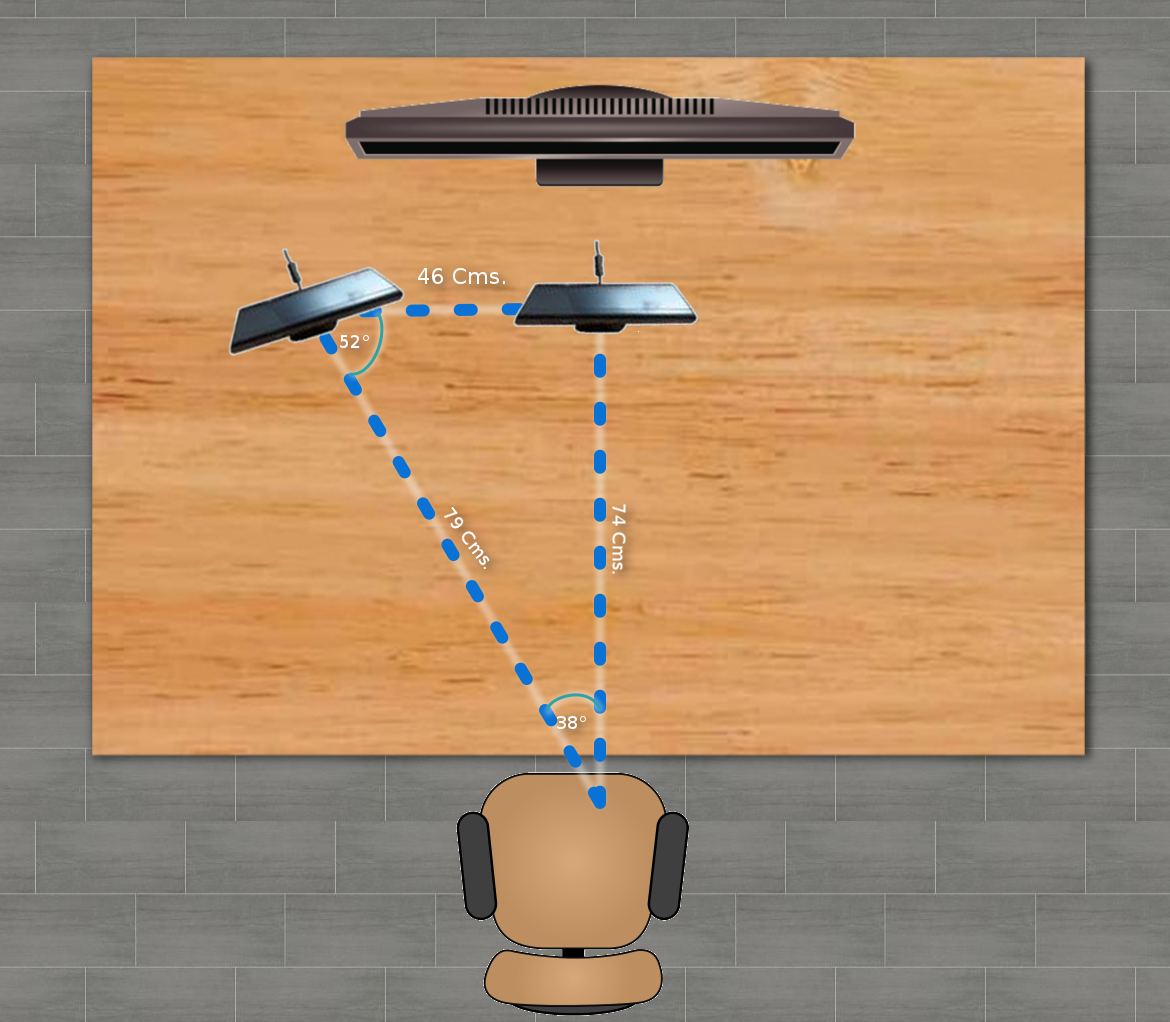
\includegraphics[scale=.2]{./Figures/system.png}
\end{center}
\caption{Configuración del sistema de reconocimiento de gestos con las manos}
\label{fig:SetupSystem}
\end{figure} 
 
una vez que le flujo de datos de los sensores de profundidad es capturado este es representado como una imagen en escala de grises de $8$ bits de $640$ p\'ixeles de ancho por $480$ p\'ixeles de largo. En las imágenes se puede apreciar detalles pequeños, es decir cambios en la profundidad de hasta $1$  $mm$ esto debido a que la escala de grises inicia cada $26$  $cm$. %creo que no se entiende bien, explicar un poco mejor.  
En la siguiente imagen se puede apreciar un ejemplo de las imágenes de profundidad. \ref{fig:ImagenCapturada}

\begin{figure}[!h]
\begin{center}
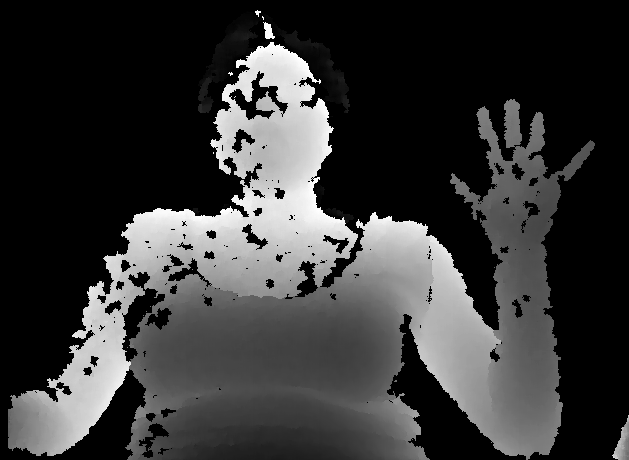
\includegraphics[scale=.5]{./Figures/166.png}
\end{center}
\caption{Representación de los datos capturados por los Kinect}
\label{fig:ImagenCapturada}
\end{figure}  

Debido a la naturaleza del funcionamiento del Kinect, las imágenes obtenidas contiene ruido del tipo (poner), el cual nos da una imagen como la figura  , el ruido  es reducido usando un filtros de mediana este es aplicado en toda la imagen en una ventada de tama\~no $13$. La imagen resultante es como la que se muestra en la figura \ref{fig:ImagenCapturada}

\begin{figure}[!h]
\begin{center}
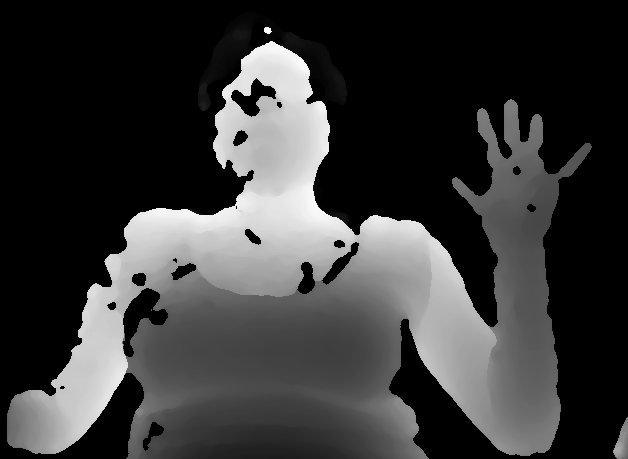
\includegraphics[scale=.5]{./Figures/166_W13.png}
\end{center}
\caption{Representación de los datos capturados por los Kinect}
\label{fig:ImagenCapturadaNoNoise}
\end{figure}  
  



%\begin{center}[a]
%\begin{tabular}{ c c c }
% cell1 & cell2 & cell3 \\ 
% cell4 & cell5 & cell6 \\  
% cell7 & cell8 & cell9    
%\end{tabular}
%\end{center}
%
%\begin{center}[b]
%\begin{tabular}{ |c|c|c| } 
% \hline
% cell1 & cell2 & cell3 \\ 
% cell4 & cell5 & cell6 \\ 
% cell7 & cell8 & cell9 \\ 
% \hline
%\end{tabular}
%\end{center}
%
%\begin{center}[c]
% \begin{tabular}{||c c c c||} 
% \hline
% Col1 & Col2 & Col2 & Col3 \\ [0.5ex] 
% \hline\hline
% 1 & 6 & 87837 & 787 \\ 
% \hline
% 2 & 7 & 78 & 5415 \\
% \hline
% 3 & 545 & 778 & 7507 \\
% \hline
% 4 & 545 & 18744 & 7560 \\
% \hline
% 5 & 88 & 788 & 6344 \\ [1ex] 
% \hline
%\end{tabular}
%\end{center}
%
%\begin{center}[d]
%\begin{tabular}{ | b{5cm} | m{2cm}| m{2cm} | } 
%\hline
%The aligning options are m for middle, p for top and b for bottom.& cell2 & cell3 \\ 
%\hline
%cell1 dummy text dummy text dummy text & cell5 & cell6 \\ 
%\hline
%cell7 & cell8 & cell9 \\ 
%\hline
%\end{tabular}
%\end{center}
%
%\begin{center}[e]
%\begin{tabular}{ |p{3cm}||p{3cm}|p{3cm}|p{3cm}|  }
% \hline
% \multicolumn{4}{|c|}{Country List} \\
% \hline
% Country Name     or Area Name& ISO ALPHA 2 Code &ISO ALPHA 3 Code&ISO numeric Code\\
% \hline
% Afghanistan   & AF    &AFG&   004\\
% Aland Islands&   AX  & ALA   &248\\
% Albania &AL & ALB&  008\\
% Algeria    &DZ & DZA&  012\\
% American Samoa&   AS  & ASM&016\\
% Andorra& AD  & AND   &020\\
% Angola& AO  & AGO&024\\
% \hline
%\end{tabular}
%\end{center}
%\begin{center}[f]
%\begin{tabular}{ |c|c|c|c| } 
%\hline
%col1 & col2 & col3 \\
%\hline
%\multirow{3}{4em}{Multiple row} & cell2 & cell3 \\ 
%& cell5 & cell6 \\ 
%& cell8 & cell9 \\ 
%\hline
%\end{tabular}
%\end{center}

\section{Detección}\label{sec:DeteccionSystem} 

En esta etapa del sistema el objetivo es localizar y segmentar la mano para poder extraer las características necesarias para el reconocimiento. 
En este trabajo se utiliza el algoritmo de detección de objetos desarrollado por (citar viola jones), como se mostró en el cap\'itulo \ref{capit:cap2} sección \ref{sec:ViolaJones}, el algoritmo  clasifica las imágenes basándose en el valor de características. 


La selección de las características se llev\'o acabo por medio del algoritmo AdaBoost; la implementaci\'on se realiz\'o utilizando el software OpenCV Haar training classifier \footnote{https://github.com/mrnugget/opencv-haar-classifier-training}. Se entren\'o con 1000 imágenes positivas (imágenes de profundidad de la mano), y 2000 negativas, (imágenes de fondo a distintas profundidades). Las imágenes positivas fueron generadas de 100 imágenes de la mano usando el software Create Samples \footnote{http://note.sonots.com/SciSoftware/haartraining.html}. Todas las imágenes usadas fueron tomadas de nuestra base de  datos \footnote{https://github.com/americamm}.

Nuestra base de datos contiene gran cantidad de imágenes de profundidad. Imágenes de fondo y de mano, estas fueron tomadas a una distancia de entre $60$ $cm$ y $200$ $cm$. Las imágenes de profundidad de la mano fueron tomadas de 6 personas distintas con tres distintas poses: palma abierta con dedos abiertos, palma abierta con dedos juntos y finalmente el pu\~no, como se muestra en la figura \ref{fig:ImagenesPoses}. Las imágenes de fondo fueron tomadas de distintos escenarios como se muestra en la figura \ref{fig:ImagenFondo}. El programa para la captura de las imágenes puede ser encontrado en github \footnote{https://github.com/americamm}.  

\begin{figure}[!h]
\begin{center}
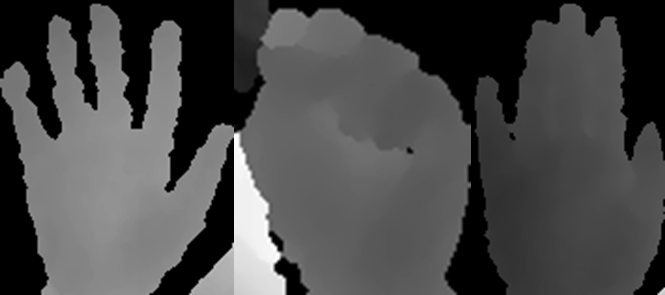
\includegraphics[scale=.5]{./Figures/TrainingImages.png}
\end{center}
\caption{Ejemplo de imágenes de la mano obtenidas de nuestra base de datos}
\label{fig:ImagenesPoses}
\end{figure}  

\begin{figure}[!h]
\begin{center}
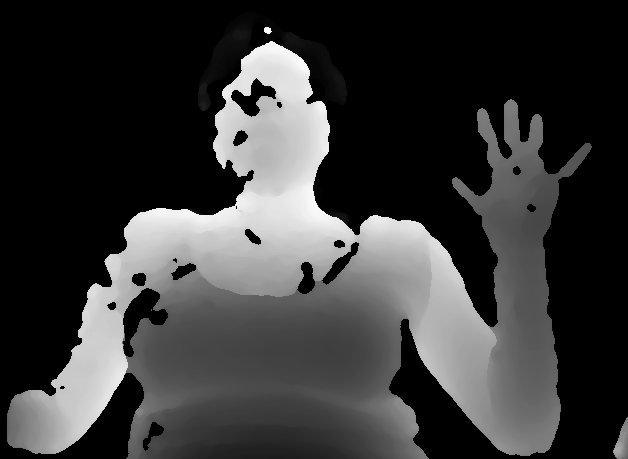
\includegraphics[scale=.5]{./Figures/166_W13.png}
\end{center}
\caption{Ejemplo de imágenes de la mano obtenidas de nuestra base de datos}
\label{fig:ImagenFondo}
\end{figure}  



%\begin{table}
%\footnotesize
%\centering
%\caption{Mauris et imperdiet     tortor. Maecenas consectetur lacus elit, dignissim eleifend dolor  ornare ut. Aenean euismod porta nisi, et volutpat ex laoreet sit amet. Sed ac elit vestibulum neque ultrices feugiat}
%\label{tab:recopilacionDeCuestionarios}
%%\rotatebox{90}{
%\begin{tabular}{m{0.2cm}m{2.5cm}m{2.5cm}m{2.5cm}m{2.5cm}m{2.5cm}}
%\hline\noalign{\smallskip}
% & \textbf{FFS} & \textbf{SOFA} & \textbf{FQ} & \textbf{CIS20R} & \textbf{FACIT}
%\\ \noalign{\smallskip}
%\hline
%\noalign{\smallskip}
%1	&	TAF	&	TAF	&	PF	&	PF	&	PF\\
%2	&	TAF	&	CM	&	CS	&	EE	&	PF\\
%3	&	PF	&	TAF	&	CS	&	CM	&	EE\\
%\hline
%\end{tabular}
%%}
%\end{table}



\section{Extracci\'on de caracter\'isticas}\label{sec:ExtraccionCaracteristicas}


%\begin{equation} \label{eq:demandaOxigeno_simple}
%\begin{split} 
%& K = R + H + V \\ 
%& R = \textrm{consumo de oxígeno} \times kg^{-1} \times min^{-1}\\ 
%& H = \textrm{constante horizontal} \times \textrm{velocidad de desplazamiento}\\ 
%& V = \textrm{constante vertical} \times \textrm{velocidad de desplazamiento}\\ 
%\end{split} 
%\end{equation} 
%
%\begin{figure}\label{eq:testing}
%\[ e = m c^2 \]
%\caption{A $ \dfrac{3}{2} $ famous equation, where $ e = m c^2  $ represent $ e = m c^2  $ energy something and $  A_{d} = -g - \frac{\sum F}{mass} $  another $\protect\pi=\protect\varpi + \protect\xi$ thing. }
%\end{figure}


\section{Reconocimiento}\label{sec:ReconocimientoSVM}



%\subsection{Extracción de parámetros}
%Ecuación \ref{eq:gravedad}. 
%
%\begin{equation} \label{eq:gravedad}
%A_{d} = -g - \frac{\sum F}{mass}
%\end{equation} 

%Donde $A_{d}$ representan la aceleración que se aplica a un dispositivo, $g$ la constante de gravedad de 9.81 m/$s^{2}$, y $\sum F$ las fuerzas que se aplican al propia sensor.

\subsection{Cálculo de la demanda de oxígeno} \label{secc:calculoDemandaOxigeno}

%Text  \ref{eq:demandaOxigeno_personalizada} and more $O_{2}$ text:
%
%\begin{equation} \label{eq:demandaOxigeno_personalizada}
%\begin{split} 
%& K = R + H + V \\ 
%& R = 3.5 - (0.0367 \times BMI) - (0.0038 \times age) + (0.1790 \times gender)\\
%& H = 0.1 \times \textrm{velocidad de desplazamiento}\\ 
%& V = 1.8 \times \textrm{velocidad de desplazamiento}\\ 
%\end{split} 
%\end{equation} 
%
%Donde $1 + 2$ representan el consumo de $O_{2}$ en reposo personalizado al usuario $(ml \times kg^{-1} \times min^{-1})$ \citep{Barstow:1991}, $H$ el componente horizontal relativo a la velocidad de desplazamiento (m/min), $V$ el componente vertical relativo a la velocidad (m/min) y pendiente de desplazamiento (\%).
%
%\begin{description}
%  \item[Velocidad:] \hfill \\
%  	Para obtener la velocidad de desplazamiento se utiliza el número de pasos realizados por el usuario como se muestra a continuación (Ecuación \ref{eq:velocidad}).
%  
%\begin{equation} \label{eq:velocidad}
%  S_{k} = D_{k}/W \hspace{10 mm} 
%  D_{k} = ST_{k} \times SL \hspace{10 mm}
%  SL = D_{total}/ST_{total} 
%\end{equation}
%\end{description}
	
\newpage
%%=====================================================

